\documentclass[12pt]{mwrep}
\usepackage{polski}
\usepackage[utf8]{inputenc}
\usepackage[T1]{fontenc}
\usepackage{times}



\usepackage[margin=20mm, left=30mm]{geometry}

%\usepackage{newtxtext}
%\usepackage{newtxmath}
\usepackage{amsmath}
\usepackage{bm}
\usepackage{mathtools}
\mathtoolsset{showonlyrefs}


\usepackage{tabularx}
\usepackage{array}
\newcolumntype{Y}{>{\centering\arraybackslash}X}
\newcolumntype{Z}{>{\centering\arraybackslash}p}
\usepackage{multirow}
\usepackage[table]{xcolor}
\usepackage{array}
\setlength\arrayrulewidth{1pt}
\newcommand{\x}{\overline{d}}
\usepackage{hyperref}


\renewcommand{\thesection}{{\hspace{-10mm}}\arabic{section}}
\renewcommand{\thesubsection}{{\hspace{-5mm}}\arabic{section}.\arabic{subsection}}

\usepackage{enumitem}
\usepackage{float}
%\usepackage{longtable}
\usepackage{graphicx}
%\usepackage{rotating}
%\usepackage{subcaption}

\newcommand{\code}[1]{\texttt{#1}}

\newcommand{\dd}{\text{d}}

%%%%%%%%%%%%%%%%%%%%%%%%%%%%%% Malec - preambuła
\usepackage{amssymb, amsfonts}






%%%%%%%%%%%%%%%%%%%%%%%%%%%%%% Budnik - preambuła
\newcommand{\indep}{\perp \!\!\! \perp}
%\usepackage{titlesec}
%\titleclass{\subsubsection}{straight}[\subsection]
%\newcounter{\subsubsection}[subsubsection]
%\renewcommand{\thesubsubsection}{{\hspace{-2mm}}\arabic{section}.\arabic{subsection}.\arabic{subsubsection}}
%\usepackage{unicode-math}
%\usepackage{dutchcal}
%\usepackage{fontspec}
%\usepackage{unicode-math}
%\setmathfont{Asana Math}
\usepackage{subfig}








\begin{document}%%%%%%%%%%%%%%%%%%%%%%%%%%%%
	\begin{center}
		{\Large\textbf{Symulacje Komputerowe}}
	\end{center}
	\begin{center}
		Raport: \textbf{1}
	\end{center}
	
	\noindent Temat sprawozdania \dotfill \textbf{Coś kreatywnego} \dotfill\dotfill\\
	Nazwisko i Imię prowadzącego kurs \dotfill \textbf{dr Michał Balcerek} \dotfill\dotfill	\newline\newline
	
	
	\noindent\begin{tabularx}{\textwidth}{|X |X|}
		\hline
		Wykonawca: & \\\hline
		\begin{center}
			Imię i Nazwisko,\\ nr indeksu
		\end{center} &  \begin{center}
			Kacper Budnik, 262286\\
			Szymon Malec, 262276
		\end{center}\\\hline
		Wydział & Wydział matematyki, W13 \\\hline
		Termin zajęć: & Wtorek,\vphantom{ $11^{1^{5}}$} $15^{15}$\\\hline
		Numer grupy ćwiczeniowej & T00-70d \\\hline
		Data oddanie sprawozdania: & \today \\\hline
		\textbf{Ocena końcowa} &\\\hline
		
	\end{tabularx}\newline\newline
	
	
	\noindent\textbf{Adnotacje dotyczące wymaganych poprawek oraz daty otrzymania poprawionego sprawozdania}
	
	
	
	\newpage

	\section{Wstęp - Koniec }
	



	\section{Liniowy generator kongruentny - Kiedyś}


%%%%%%%%%%%%%%%%%%%%%%%%%%%%%%%%%%%%%%%%1
	
	\section{Metoda odwrotnej dystrybuanty - Malec}
	
	\subsection{Opis}
	\noindent Metoda ta polega na generowaniu zmiennej losowej $X$ generując zmienną $U$ z rozkładu jednostajnego oraz nakładając na nią funkcję odwrotną dystrybuanty.
	\subsubsection{Algorytm dla rozkładów dyskretnych}
	\noindent Załóżmy, że rozkład $X$ ma postać $\mathrm{P}(X = x_i) = p_\mathrm{i}$, \ $i = 1, 2,\dots $.
	\begin{enumerate}[leftmargin=10mm]
		\item Generuj $U \sim \mathcal{U}(0, 1)$.
		\item Wyznacz $j \in \mathbb{N} $ takie, że $ \sum\limits_{i=1}^{j-1} p_i < U \leqslant \sum\limits_{i=1}^{j} p_i $.
		\item Zwróć $ X = x_i $.
	\end{enumerate}
	\subsubsection{Algorytm dla rozkładów ciągłych}
	\noindent Załóżmy, że $X$ ma dystrybuantę $F(x)$.
	\begin{enumerate}[leftmargin=10mm]
		\item[a)] Jeśli dystrybuanta jest ściśle rosnąca:
		\begin{enumerate}
			\item[1.] Generuj $U \sim \mathcal{U}(0, 1)$.
			\item[2.] Zwróć $ X = F_X^{-1}(U) $.
		\end{enumerate}
		\item[b)] Jeśli dystrybuanta nie jest ściśle rosnąca:
		\begin{enumerate}
			\item[1.] Generuj $U \sim \mathcal{U}(0, 1)$.
			\item[2.] Zwróć $ X = \widetilde{F}_X^{-1}(U) $, gdzie $ \widetilde{F}_X^{-1}(y) = \mathrm{inf}\{x \in \mathbb{R}: F_X(x) \geqslant y\} $.
		\end{enumerate}
	\end{enumerate}

	\subsection{Przykłady}
	
	\subsubsection{Dyskretny - rozkład Poissona}
	\noindent Celem jest wygenerowanie $X \sim \mathcal{Poiss}(\lambda)$. Przypomnijmy jak wygląda rozkład Poisson:
	$$ p_i = \mathrm{P}(X = i) = \mathrm{e}^{-\lambda} \frac{\lambda^i}{i!}. $$
	Algorytm będzie więc polegał na generowaniu $U \sim \mathcal{U}(0, 1)$ i wyznaczaniu $j \in \mathbb{N} $ takiego, że 
	$$ \sum\limits_{i=1}^{j-1} p_i < U \leqslant \sum\limits_{i=1}^{j} p_i. $$
	Zauważmy, że
	$$ p_{i + 1} = p_i \cdot \frac{\lambda}{i + 1}. $$
	
	\subsubsection{Ciągły - rozkład Cauchy'ego}
	\noindent Chcemy wygenerować $ X \sim \mathcal{C}(\mu, \sigma) $. 
	Dystrybuanta rozkładu Cauchy'ego ma postać
	$$ F(x) = \frac{1}{\pi} \arctan{\left(\frac{x - \mu}{\sigma}\right)} + \frac{1}{2}. $$
	Za pomocą elementarnych przekształceń jesteśmy w stanie otrzymać funkcję odwrotną
	$$ F^{-1}(y) = \sigma \tan \left(\pi \left(y - \frac{1}{2}\right) \right) + \mu. $$
	Zatem, żeby wygenerować $X$, należy najpierw wygenerować $U \sim \mathcal{U}(0, 1) $ i zwrócić $F^{-1}(U)$. Możemy to jednak lekko uprościć. Niech $ V \sim \mathcal{U}\left(-\frac{\pi}{2}, \frac{\pi}{2}\right) $. Wtedy
	$$ V \buildrel{d}\over{=} \pi \left(U - \frac{1}{2}\right). $$
	Ostatecznie algorytm będzie wyglądał następująco:
	\begin{enumerate}[leftmargin=10mm]
		\item Generuj $V \sim \mathcal{U}\left(-\frac{\pi}{2}, \frac{\pi}{2}\right)$.
		\item Zwróć $ X = \sigma \tan(V) + \mu $.
	\end{enumerate}
	Aby przetestować powyższy algorytm, generujemy wektor 1000 realizacji zmiennej $X$, a następnie porównujemy dystrybuantę empiryczną tej próbki z dystrybuantą teoretyczną oraz tworzymy histogram i porównujemy go z gęstością.
	%\includegraphics[scale=1]{plot3.png}
	Jak możemy zauważyć dystrybuanty empiryczna i teoretyczna są do siebie zbliżone. To samo możemy powiedzieć o krzywej gęstości, której kształt jest podobny do histogramu próby.


%%%%%%%%%%%%%%%%%%%%%%%%%%%%%%%%%%%%%%%%2

	
	\section{Metoda akceptacji i odrzucenia\textsuperscript{\cite{AO - dyskretny}} - Budnik}
	\subsection{Opis metody dla przypadku dyskretnego\textsuperscript{\cite{AO - dyskretny}}}
	Metoda akceptacji i odrzucenia służy do generowania zmiennej losowej $X$ przy użyciu innych zmiennych. By móc wykorzystać tą metodę muszą być spełnione:
	\begin{itemize}[leftmargin=10mm]
		\item Potrafimy efektywnie generować inną zmienną losową $Y$
		\item Zmienne $X$ oraz $Y$ muszą być skupione na tym samym zbiorze
		\item Potrafimy wyznaczyć stałą $c$ taką że $\dfrac{\mathrm{P}(X=i)}{\mathrm{P}(Y=i)}=\dfrac{p_Y}{q_Y}\leqslant c$ dla każdego $i$
	\end{itemize}
	Jeśli są spełnione powyższe założenia możemy użyć poniższego algorytmu do generowania zmiennej $X$.
	\subsubsection{Algorytm}
	\begin{enumerate}[leftmargin=10mm]
		\item Generuj jedną realizację $Y$
		\item Generuj $U\sim \mathcal{U}(0,1)$, $U\indep Y$
		\item Jeśli $U\leqslant\frac{p_Y}{cq_Y}$ zwróć $X=Y$, w przeciwnym wróć do 1.
	\end{enumerate}
	
	
	\subsection{Opis metody dla przypadku ciągłego\textsuperscript{\cite{AO - ciagly}}}
	Metoda akceptacji i odrzucenia służy do generowania zmiennej losowej $X$ o gęstości $f(x)$ przy użyciu innych zmiennych. By móc wykorzystać tą metodę muszą być spełnione:
	\begin{itemize}[leftmargin=10mm]
		\item Potrafimy efektywnie generować inną zmienną losową $Y$ o gęstości $g(x)$
		\item Zmienne $X$ oraz $Y$ muszą być skupione na tym samym zbiorze
		\item Potrafimy wyznaczyć stałą $c$ taką że $\sup\dfrac{f(x)}{g(x)}\leqslant c$ dla każdego $x$, gdzie $g(x)\neq0$ (więc również $f(x)\neq0$)
	\end{itemize}
	\subsubsection{Algorytm}
	\begin{enumerate}[leftmargin=10mm]
		\item Generuj jedną realizację $Y$
		\item Generuj $U\sim \mathcal{U}(0,1)$, $U\indep Y$
		\item Jeśli $U\leqslant\dfrac{f(Y)}{cg(Y)}$ zwróć $X=Y$, w przeciwnym wróć do 1.
	\end{enumerate}

	\subsection{Szybkość algorytmu}
	W obu przypadkach, ciągłym i dyskretnym, prawdopodobieństwo, że zmienna zostanie zaakceptowana wynosi $\frac{1}{c}$.\\
%	Średnia liczba powtórzeń algorytmu wynosi $c$, zatem stałą tę powinniśmy dobierać jak najmniejszą spełniającą wymagane kryteria.
	Liczba iteracji algorytmu potrzebnych do wygenerowania zmiennej ma rozkład $\mathcal{G}eom(\frac{1}{c})$, zatem średnia liczba iteracji potrzebna do wygenerowania tej zmiennej to $c$. Z tego powodu stałą tą powinniśmy dobrać jak najmniejszą możliwą. Najoptymalniej wybrać $c=\max\frac{p_Y}{q_Y}$ w przypadku dyskretnym oraz $c=\sup\frac{f(x)}{g(x)}$ dla przypadku ciągłego.
%		Prawdopodobieństwo że zmienna zostanie zaakceptowana wynosi
%	$$\mathbb{P}(\text{'wartość zaakceptowana'})=\frac{1}{c}$$
%	zatem by algorytm był wydajny stała $c$ powinna być jak najmniejsza. Średnia liczba powtórzeń algorytmu wynosi $c$.

	\subsection{Przykłady}
	
	\subsubsection{Dyskretny}
	Niech $X$ ma następujący rozkład
	\begin{equation}
		\mathrm{P}(X=i)=\begin{cases}
			0.1, \quad\text{dla $i=-2$}\\
			0.2, \quad\text{dla $i=-1$}\\
			0.5, \quad\text{dla $i=\phantom{-}0$}\\
			0.2, \quad\text{dla $i=\phantom{-}1$}\\
%			0.1, \phantom{0}\quad\text{dla $i=\phantom{-}1$}
		\end{cases}
	\end{equation}
	Do generowania tej zmiennej potrzebujemy zmienną, która jest skupiona na tym samym zbiorze. Najprostszym pomysłem jest wykorzystanie zmiennej z rozkładu jednostajnego dyskretnego $Y\sim\mathcal{DU}(-2,-1,0,1)$. Prawdopodobieństwo, że $Y$ przyjmie daną wartość stale wynosi $\frac{1}{4}$, zatem łatwo wyliczyć stałą $c=4\max_i\mathrm{P}(X=i)=4\cdot0.5=2$. Znając tą stałą wystarczy zastosować dany algorytm
	\begin{enumerate}[leftmargin=10mm]
		\item Generuj jedną realizację $Y\sim\lfloor4\cdot\mathcal{U}(0,1)\rfloor-2$
		\item Generuj $U\sim \mathcal{U}(0,1)$, $U\indep Y$
		\item Jeśli $U\leqslant2p_Y$ zwróć $X=Y$, w przeciwnym wróć do 1.
	\end{enumerate}
	\begin{figure}[H]\caption{Sprawdzenie poprawności metody Akceptacji-Odrzucenie dla próby o rozmiarze $n=100$}\label{fig:AO_dysk}
		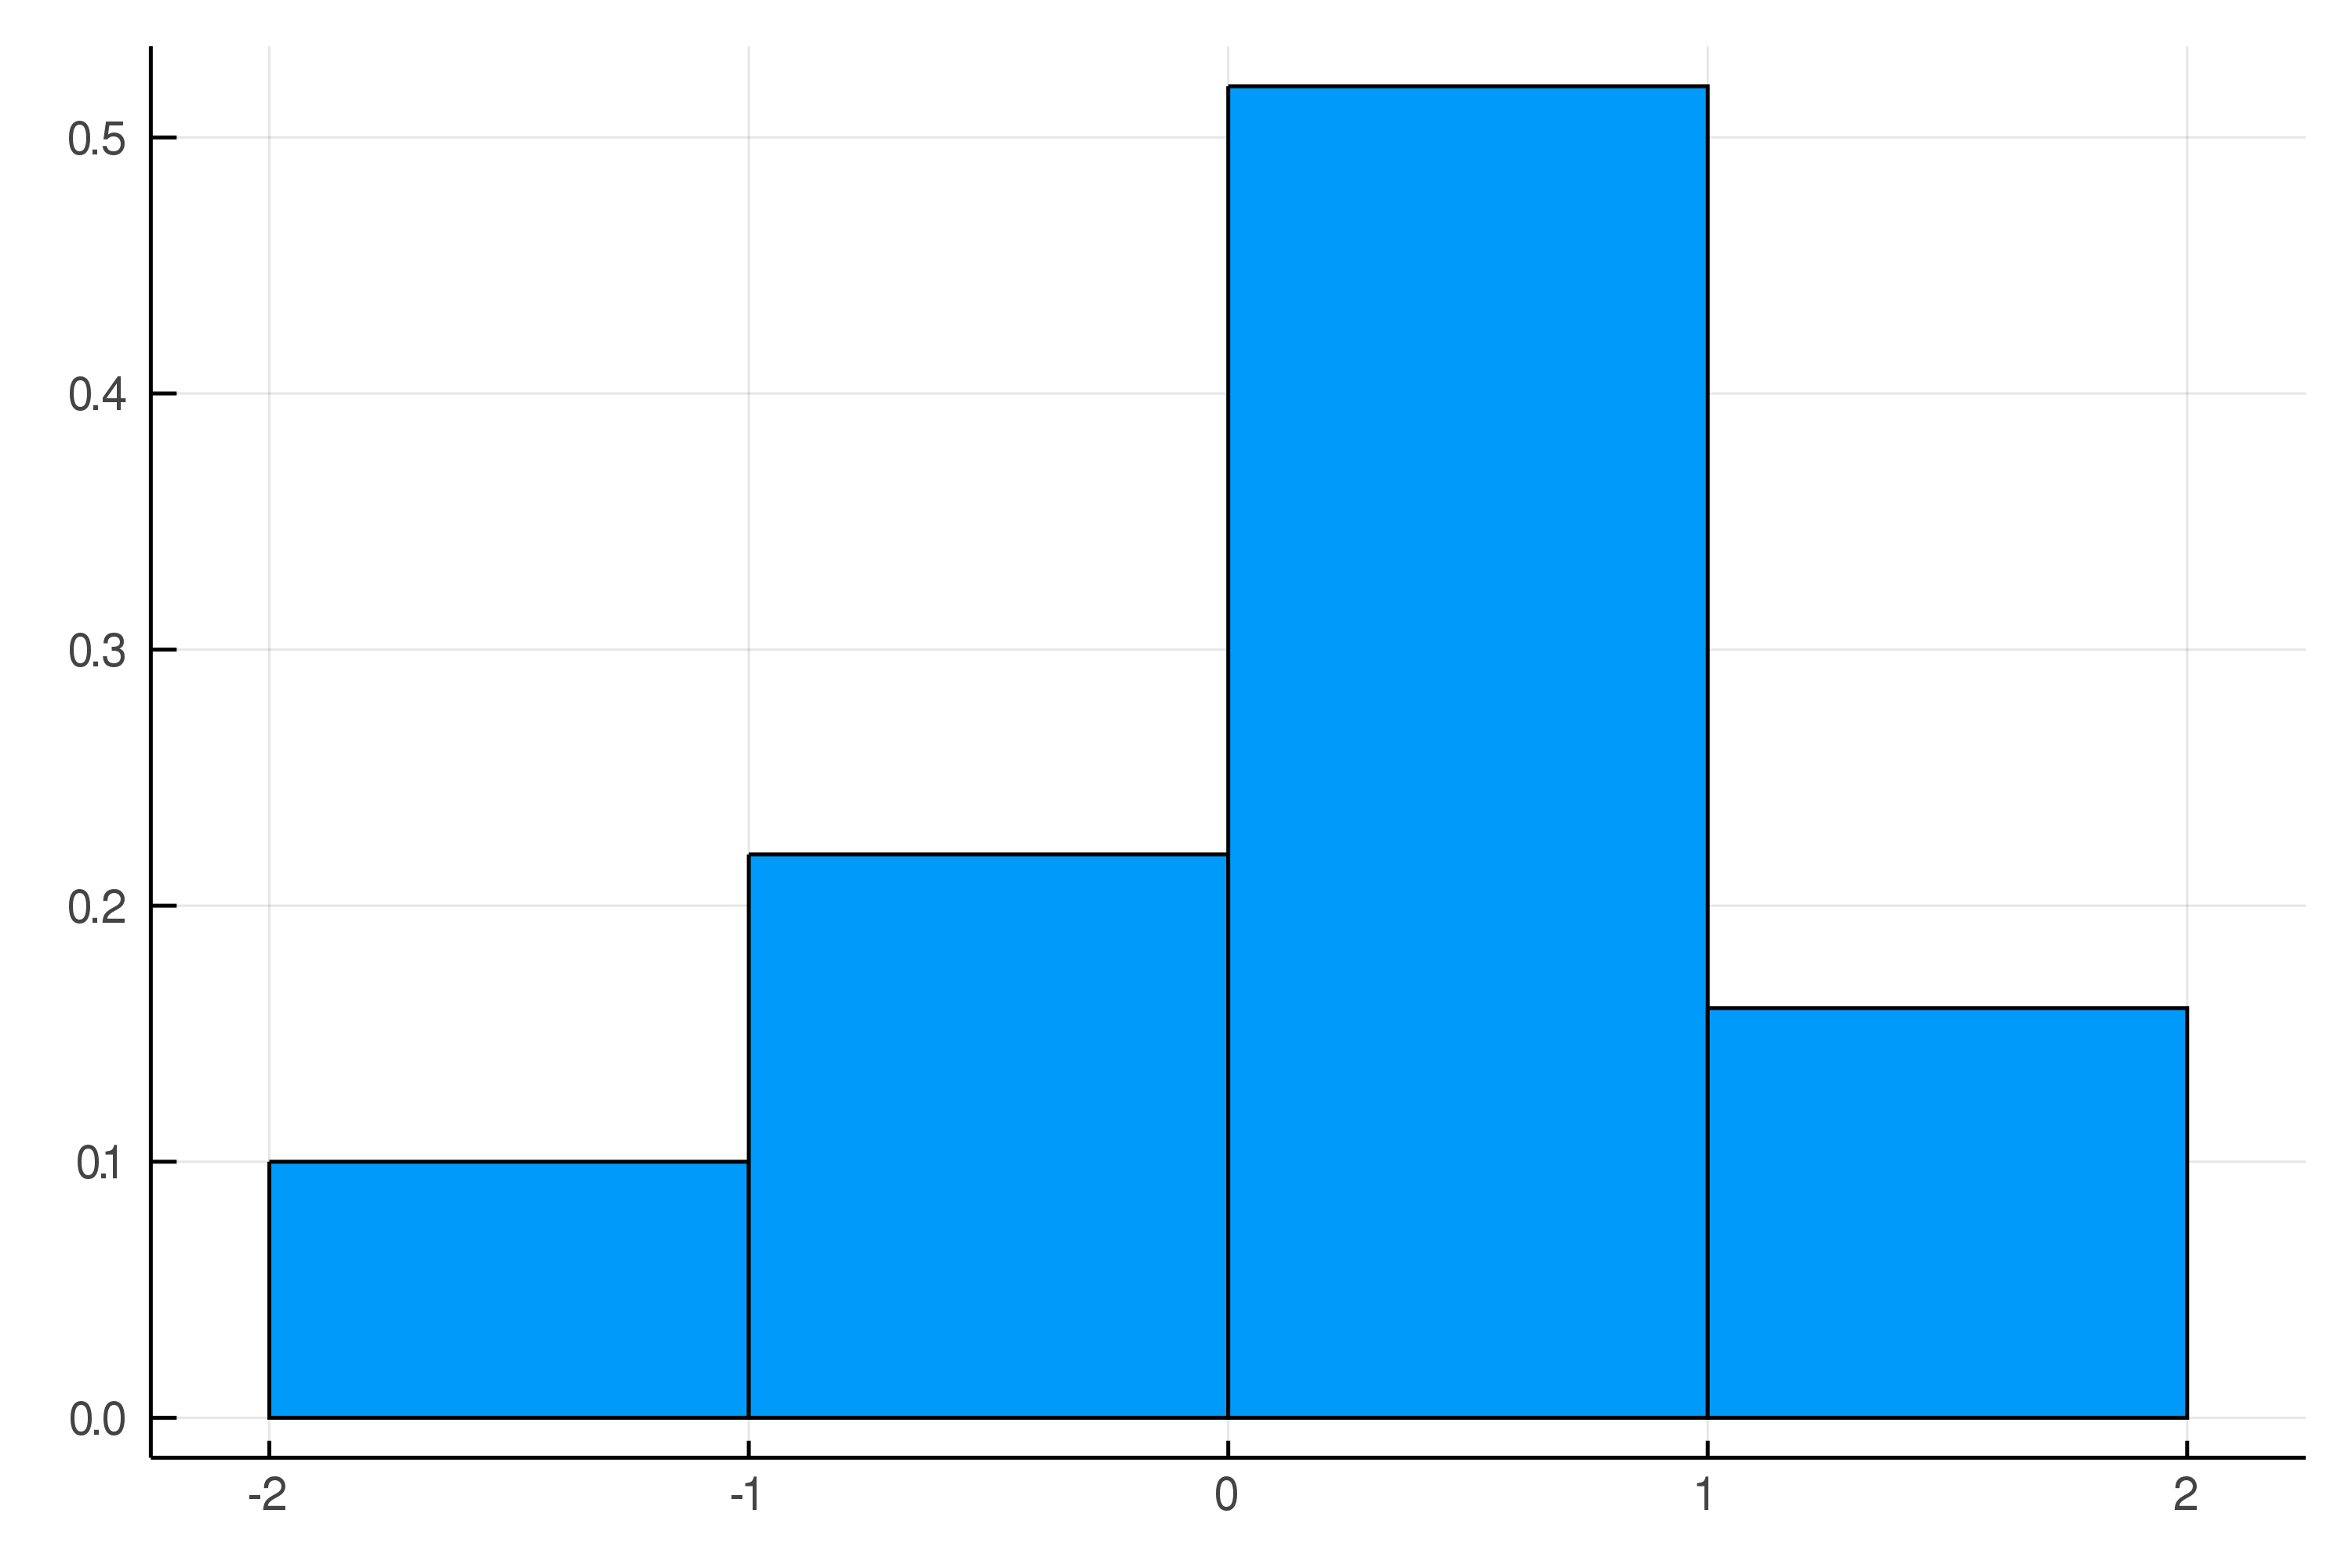
\includegraphics[width=\columnwidth]{fig/fig_AO_dysk.png}
	\end{figure}
	
	
%	Możemy zauważyć, że nasza zmienna ma rozkład skupiony na wym samym zbiorze co $Y=Z-2$, gdzie $Z\sim\mathcal{B}(n=4,p)$. Zmienną $Z$ potrafimy już efektywnie generować przy pomocy metody splotowej. Ale są szybsze sposoby i ten podobny do tego wykonywaliśmy już na zajęciach, ale wszystkie są takie same.
 
 	\subsubsection{Ciągły}
 	Chcemy wygenerować zmienną $X$ o gęstości $f(x)= \ln(2)\cdot\sin(x)\cdot2^{\cos(x)}\boldmath 1_{(0,\frac{\pi}{2})}$. Użyjemy do tego zmiennej $Y\sim\mathcal{U}(0,\frac{\pi}{2})$ o funkcji gęstości $g(x)=\frac{2}{\pi}\boldmath 1_{(0,\frac{\pi}{2})}$. Zaczniemy od wyliczenia stałej $c$.
 	\begin{equation}
 		c=\sup\limits_{x\in(0,\frac{\pi}{2})}\frac{f(x)}{g(x)}=\sup\limits_{x\in(0,\frac{\pi}{2})}\sin(x)\cdot2^{\cos(x)}\cdot\frac{\pi\ln(2)}{2}\approx \frac{4}{3}
 	\end{equation}
 	Teraz wystarczy się stosować do następującego algorytmu, czyli
	\begin{enumerate}[leftmargin=10mm]
		\item Generuj $Y\sim \frac{\pi}{2}\mathcal{U}(0,1)$
		\item Generuj $U\sim \mathcal{U}(0,1)$, $U\indep Y$
		\item Jeśli $U\leqslant\sin(Y)\cdot2^{\cos(Y)}\cdot\dfrac{3\pi\ln(2)}{8}$ zwróć $X=Y$, w przeciwnym wróć do 1.
	\end{enumerate}	
%	Stosując się do powyższego algorytmu wygenerowaliśmy próbę rozmiaru $n=10^6$. By sprawdzić, czy nasza metoda jest poprawna na poniższych wykresach porównaliśmy gęstość rozkładu z histogramem wygenerowanej próby oraz dystrybuanty: empiryczną z teoretyczną. 
 	

	\begin{figure}[H]\caption{Sprawdzenie poprawności metody Akceptacji-Odrzucenie dla próby o rozmiarze $n=1000$}\label{fig:AO_con}
		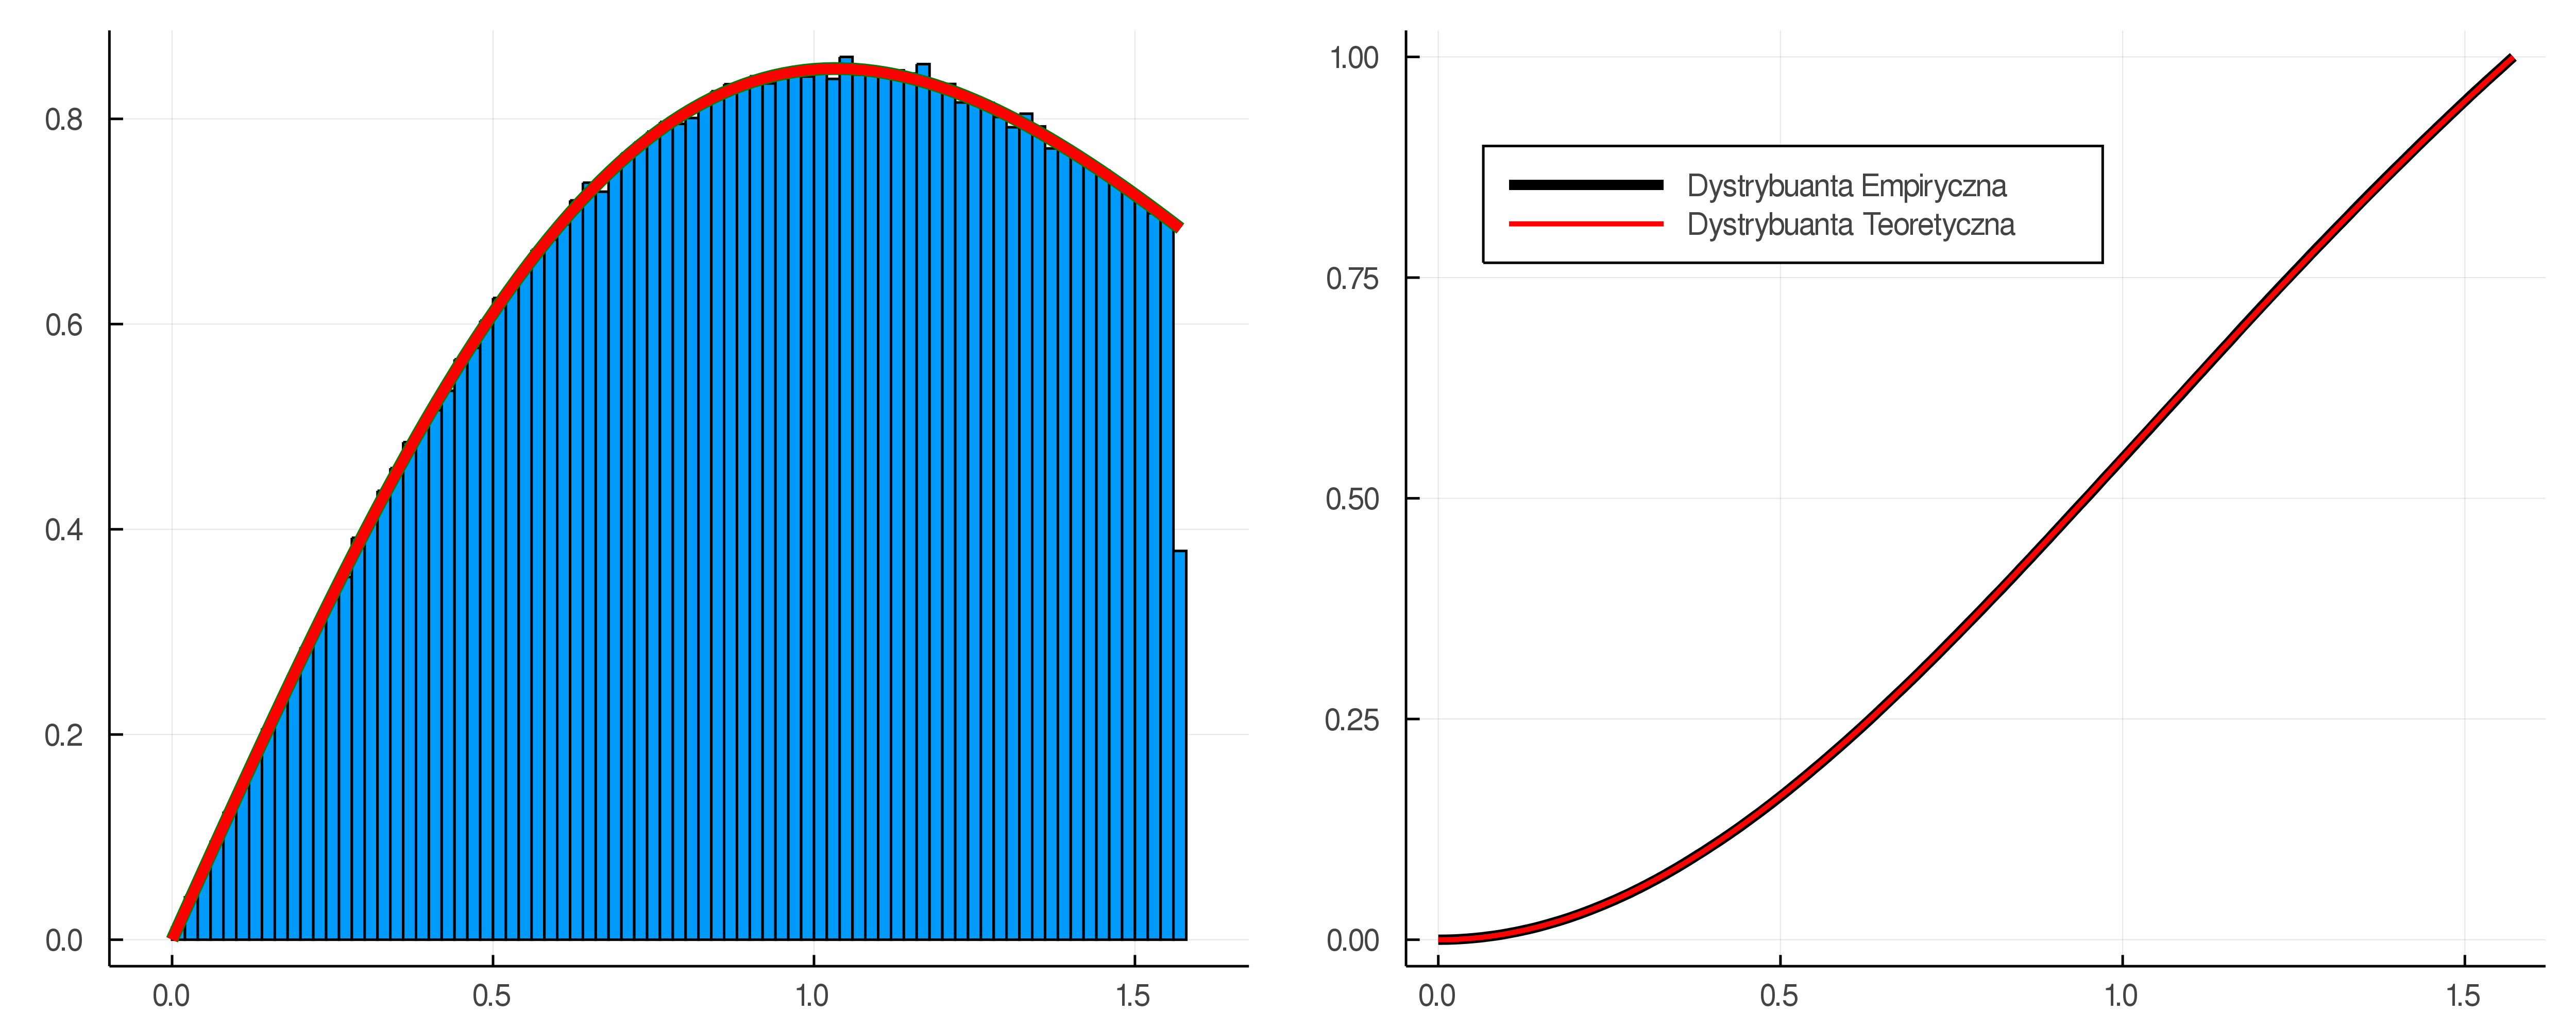
\includegraphics[width=\columnwidth]{fig/fig_AO_con.png}
	\end{figure}
	
%	\begin{figure}[H]\caption{Porównanie na wykresach wygenerowanej }
%		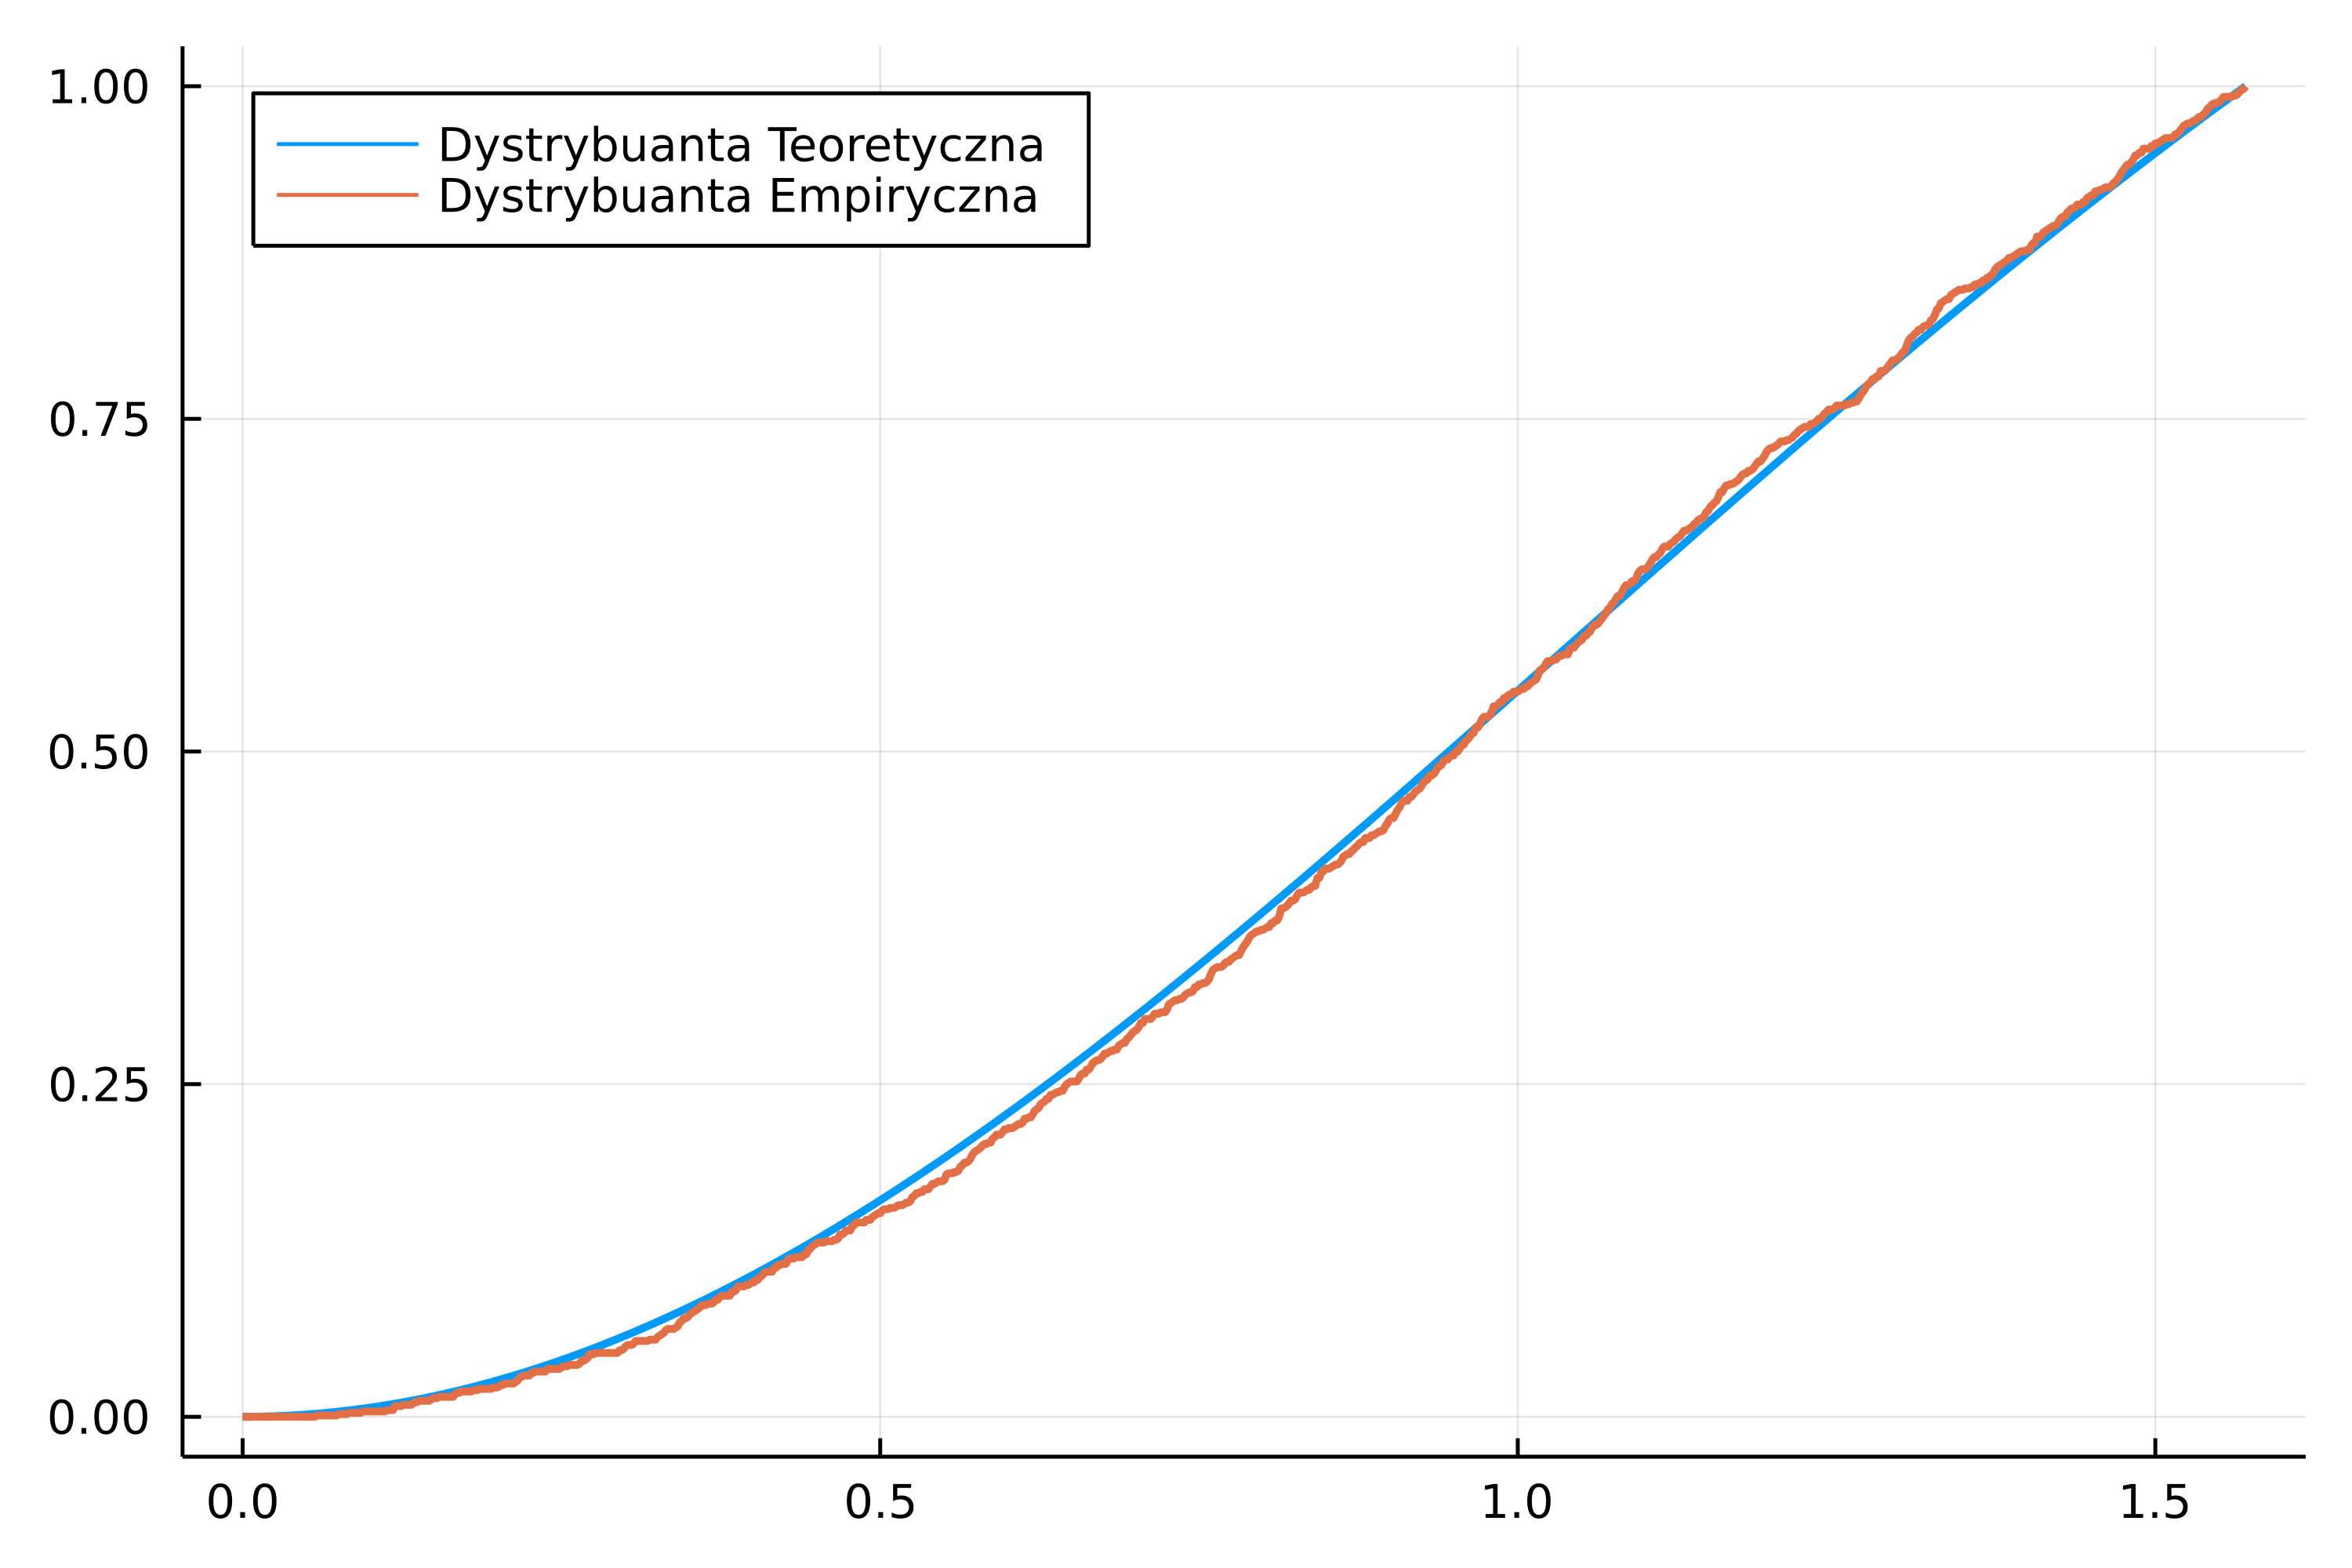
\includegraphics[width=\columnwidth]{fig/fig_AO_con_cdf.png}
%	\end{figure}
%
%	\begin{figure}[H]
%		\centering
%		\subfloat[\centering label 1]{{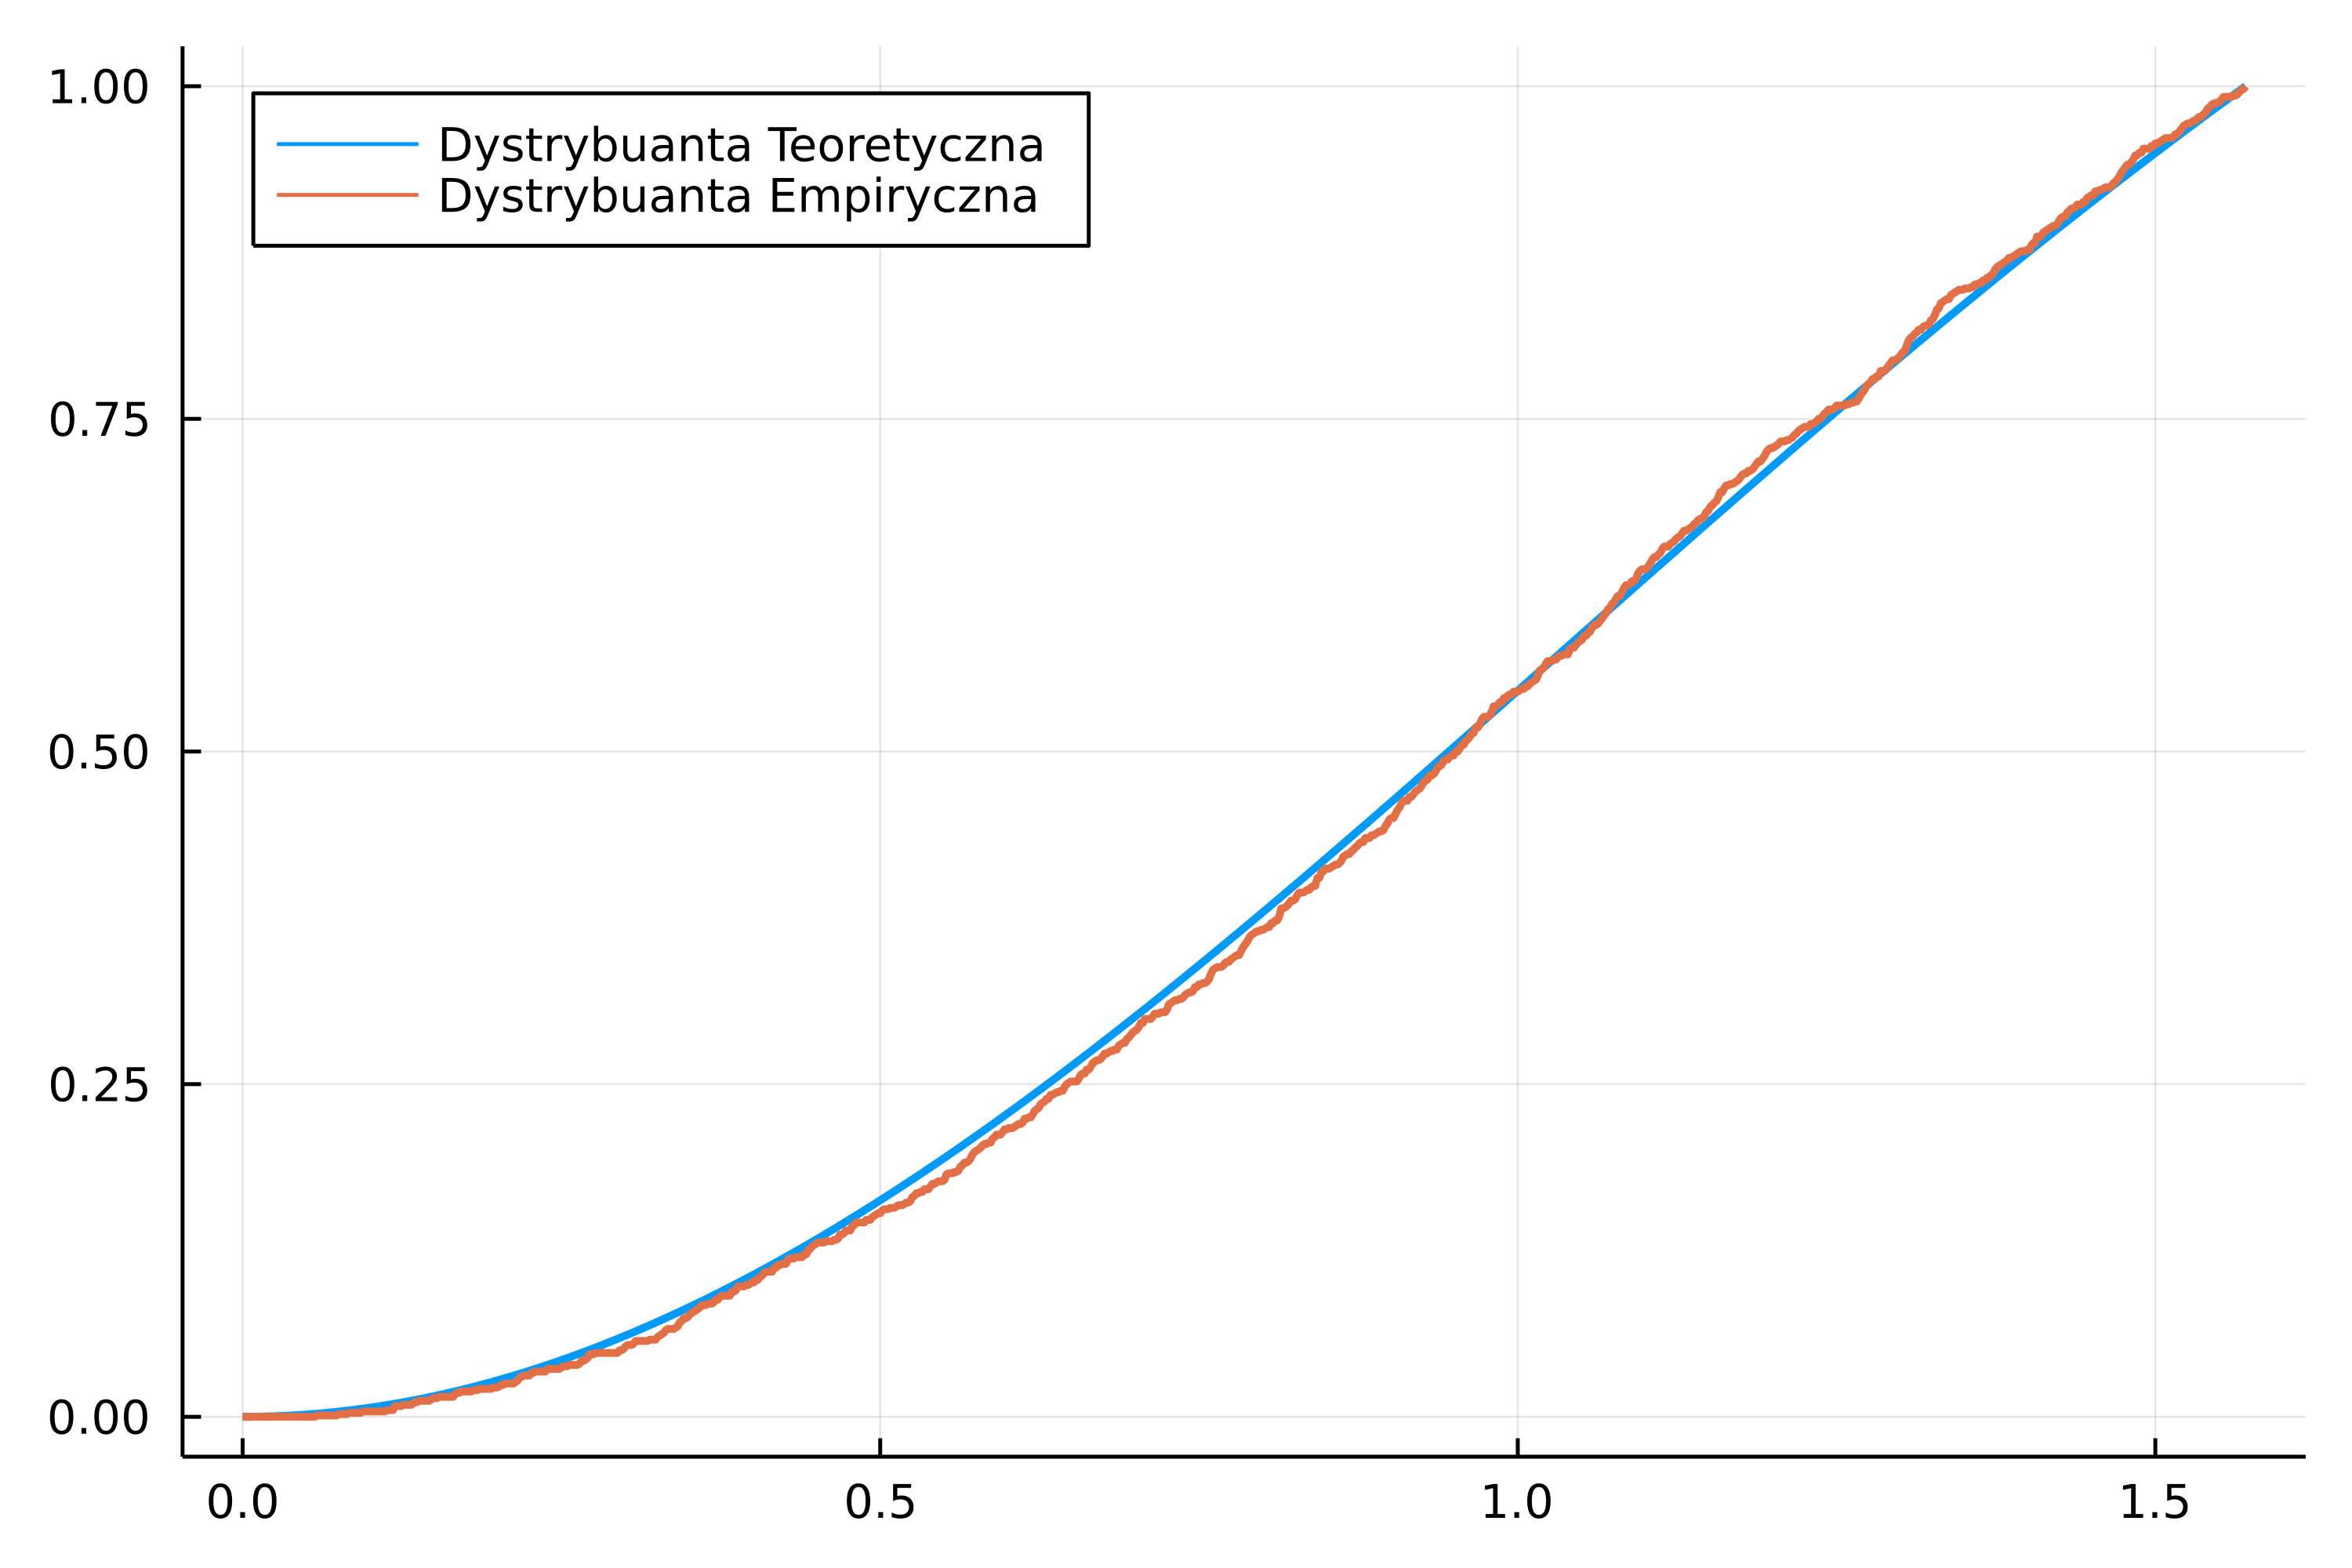
\includegraphics[width=\columnwidth/2-10mm]{fig/fig_AO_con_cdf.png} }}%
%		\qquad
%		\subfloat[\centering label 2]{{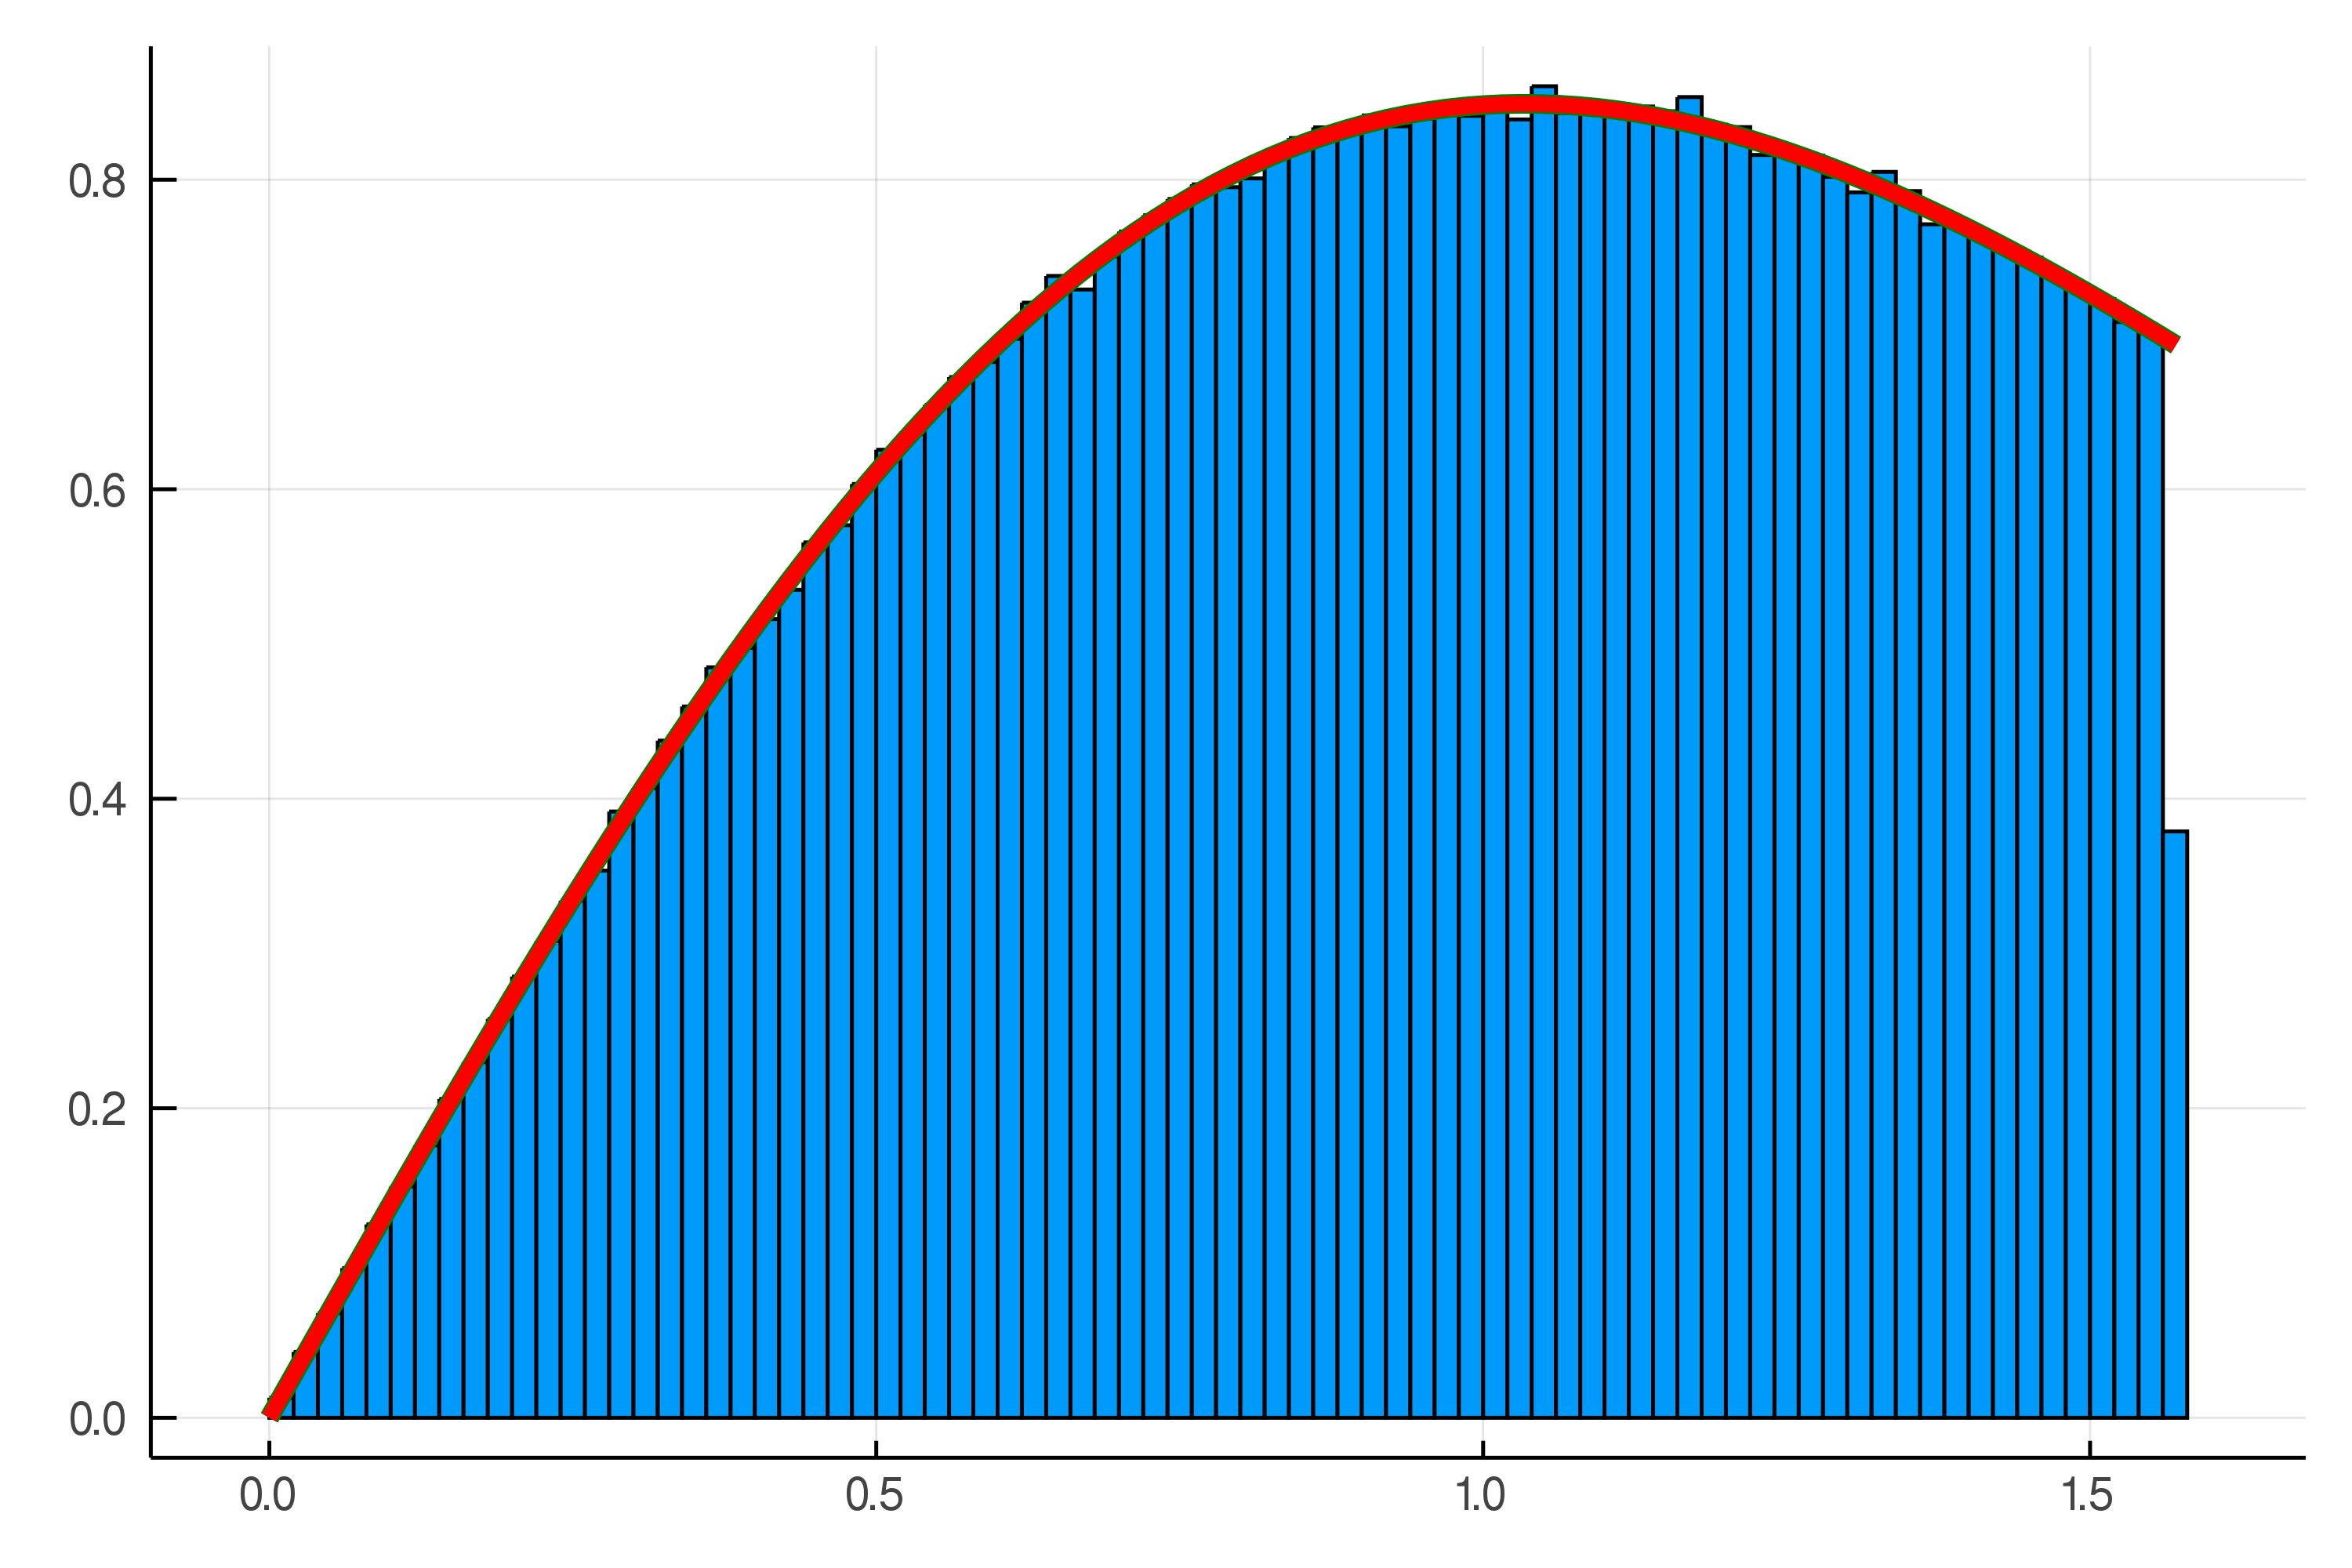
\includegraphics[width=\columnwidth/2-10mm]{fig/fig_AO_con_hist.png} }}%
%		\caption{2 Figures side by side}%
%		\label{fig:example}%
%	\end{figure}









%%%%%%%%%%%%%%%%%%%%%%%%%%%%%%%%%%%%%%%%3
	
	\section{Metoda splotowa - Malec}
	
	\subsection{Opis}
	\noindent Metoda ta pozwala wygenerować pewną zmienną losową $X$, przy pomocy innych zmiennych, które potrafimy efektywnie generować, i zsumowaniu ich. Załóżmy, że
	$$ X \buildrel{d} \over{=} Y_1 + Y_2 + \dots + Y_n, $$
	gdzie $Y_i$ to zmienne losowe niezależne. Wtedy algorytm wygląda następująco:
	\begin{enumerate}
		\item Generuj $ Y_1, Y_2, \dots, Y_n $.
		\item Zwróć $ X = Y_1 + Y_2 + \dots + Y_n $.
	\end{enumerate}

	\subsection{Przykłady}
	
	\subsubsection{Dyskretny - rozkład dwumianowy}
	\noindent Niech $ X \sim \mathcal{B}(n, p) $ oraz niech $Y_1, Y_2, \dots, Y_n$ będzie ciągiem niezależnych zmiennych losowych będących wynikami prób Bernoulliego z prawdopodobieństwem sukcesu $p$. Wtedy
	$$ X \buildrel{d} \over{=} Y_1 + Y_2 + \dots + Y_n. $$
	Stąd mamy algorytm:
	\begin{enumerate}[leftmargin=10mm]
		\item Generuj $ Y_1, Y_2, \dots, Y_n $, gdzie $Y_i \sim \mathcal{B}(1, p) $.
		\item Zwróć $ X = Y_1 + Y_2 + \dots + Y_n $.
	\end{enumerate}
	
	\subsubsection{Ciągły - rozkład chi-kwadrat}
	\noindent Niech $ X \sim \mathcal{X}^2(n) $ oraz niech $Y_1, Y_2, \dots, Y_n$ będzie ciągiem niezależnych zmiennych losowych o rozkładzie normalnym standardowym. Wtedy
	$$ X \buildrel{d} \over{=} Y_1^2 + Y_2^2 + \dots + Y_n^2. $$
	Stąd otrzymujemy algorytm:
	\begin{enumerate}[leftmargin=10mm]
		\item Generuj $ Y_1, Y_2, \dots, Y_n $, gdzie $Y_i \sim \mathcal{N}(0, 1) $.
		\item Zwróć $ X = Y_1^2 + Y_2^2 + \dots + Y_n^2 $.
	\end{enumerate}
	
	
	
	
	
	\section{Metoda kompozycji - Malec}
	
	\subsection{Opis}
	\noindent Metoda ta służy do generowania wyłącznie ciągłych rozkładów. Załóżmy, że zmienna losowa $X$, którą chcemy symulować, ma dystrybuantę postaci
	$$ F(x) = \sum_{i=1}^n p_i F_i(x), $$
	gdzie $p_i > 0$, \ $\sum\limits_{i=1}^n p_i = 1$ oraz $F_i$ to dystrybuanty pewnych zmiennych losowych $Y_i$. Jeżeli zmienne $Y_i$ mają gęstość, to równoważne będzie założenie, że gęstość zmiennej $X$ ma postać
	$$ f(x) = \sum_{i=1}^n p_i f_i(x), $$
	gdzie $f$ są gęstościami zmiennych $Y_i$. Do wygenerowania $X$ może posłużyć poniższy algorytm:
	\begin{enumerate}[leftmargin=10mm]
		\item Generuj zmienną losową $I$ o rozkładzie $\mathrm{P}(I = i) = p_i$.
		\item Generuj $Y_I$.
		\item Zwróć $X = Y_I$.
	\end{enumerate}

	\subsection{Przykład}
	\noindent Chcemy wygenerować zmienną losową $X$ o dystrybuancie
	$$ F(x) = \frac{1}{3\pi}\arctan(x) - \frac{2}{3}\mathrm{e}^{-2x} + \frac{5}{6}. $$
	Jeśli zapiszemy ją w postaci
	$$ F(x) = \frac{1}{3}\left(\frac{1}{\pi}\arctan(x) + \frac{1}{2}\right) + \frac{2}{3}\left(1 - \mathrm{e}^{-2x}\right), $$
	to możemy zauważyć, że jest to suma dystrybuant rozkładów Cauchy'ego i wykładniczego. Weźmy zatem $Y_1 \sim \mathcal{C}(0, 1)$ oraz $Y_2 \sim \mathcal{Exp}(2)$. Niech $p_1 = \frac{1}{3}$ i $p_2 = \frac{2}{3}$. Wtedy możemy zapisać
	$$ F(x) = p_1 F_1(x) + p_2 F_2(x), $$
	gdzie $F_1$ i $F_2$ to dystrybuanty odpowiednio $Y_1$ i $Y_2$. Stąd algorytm prezentuje się następująco:
	\begin{enumerate}[leftmargin=10mm]
		\item Generuj $I$ o rozkładzie $\mathrm{P}(I = 1) = \frac{1}{3}$, \ $\mathrm{P}(I = 2) = \frac{2}{3}$.
		\item Generuj $Y_I$.
		\item Zwróć $X = Y_I$.
	\end{enumerate}



%%%%%%%%%%%%%%%%%%%%%%%%%%%%%%%%%%%%%%%%4
	
	\section{Metoda Boxa-M{\"u}llera\textsuperscript{\cite{box-kox}} - Budnik}
	\subsection{Opis}
	Najważniejszym rozkładem w prawdopodobieństwie jest rozkład normalny. Dlatego istnieje specjalna metoda generowania jego. Łatwo można pokazać (co zrobiliśmy na kursie Modelowanie Stochastyczne), że jeśli $U_1,U_2$ - iid, $U_1\sim\mathcal{U}(0,1)$, to zmienne
	\begin{equation}\label{eq:B-M}
		\begin{split}
			X=\sqrt{-2\ln(U_1)}\cos(2\pi U_2)\\
			Y=\sqrt{-2\ln(U_1)}\sin(2\pi U_2)
		\end{split}
	\end{equation}
	są niezależne oraz obie mają rozkład normalny standardowy $\mathcal{N}(0,1)$. Na tej podstawie powstał poniższy algorytm
	\subsubsection{Algorytm}
	\begin{enumerate}[leftmargin=10mm]
		\item Generuj zmienne $U_1, U_2$ - iid, $U_1\sim\mathcal{U}(0,1)$
		\item Zwróć:
		\begin{equation}
			\begin{split}
				X=\sqrt{-2\ln(U_1)}\cos\left(2\pi U_2\right)\\
				Y=\sqrt{-2\ln(U_1)}\sin\left(2\pi U_2\right)
			\end{split}
		\end{equation}
	\end{enumerate}
	Algorytm ten generuje od razu dwie próby z rozkładu normalnego standardowego. By wygenerować zmienną z rozkładu $\mathcal{N}(\mu,\sigma^2)$ wystarczy wcześniej wygenerowane zmienne pomnożyć przez $\sigma$ po czym dodać do nich $\mu$.
	\subsection{Przykłady}
	
	\begin{figure}[H]\caption{Sprawdzenie poprawności metody Boxa-M\"ullera dla próby o rozmiarze $n=1000$}\label{fig:BM}
		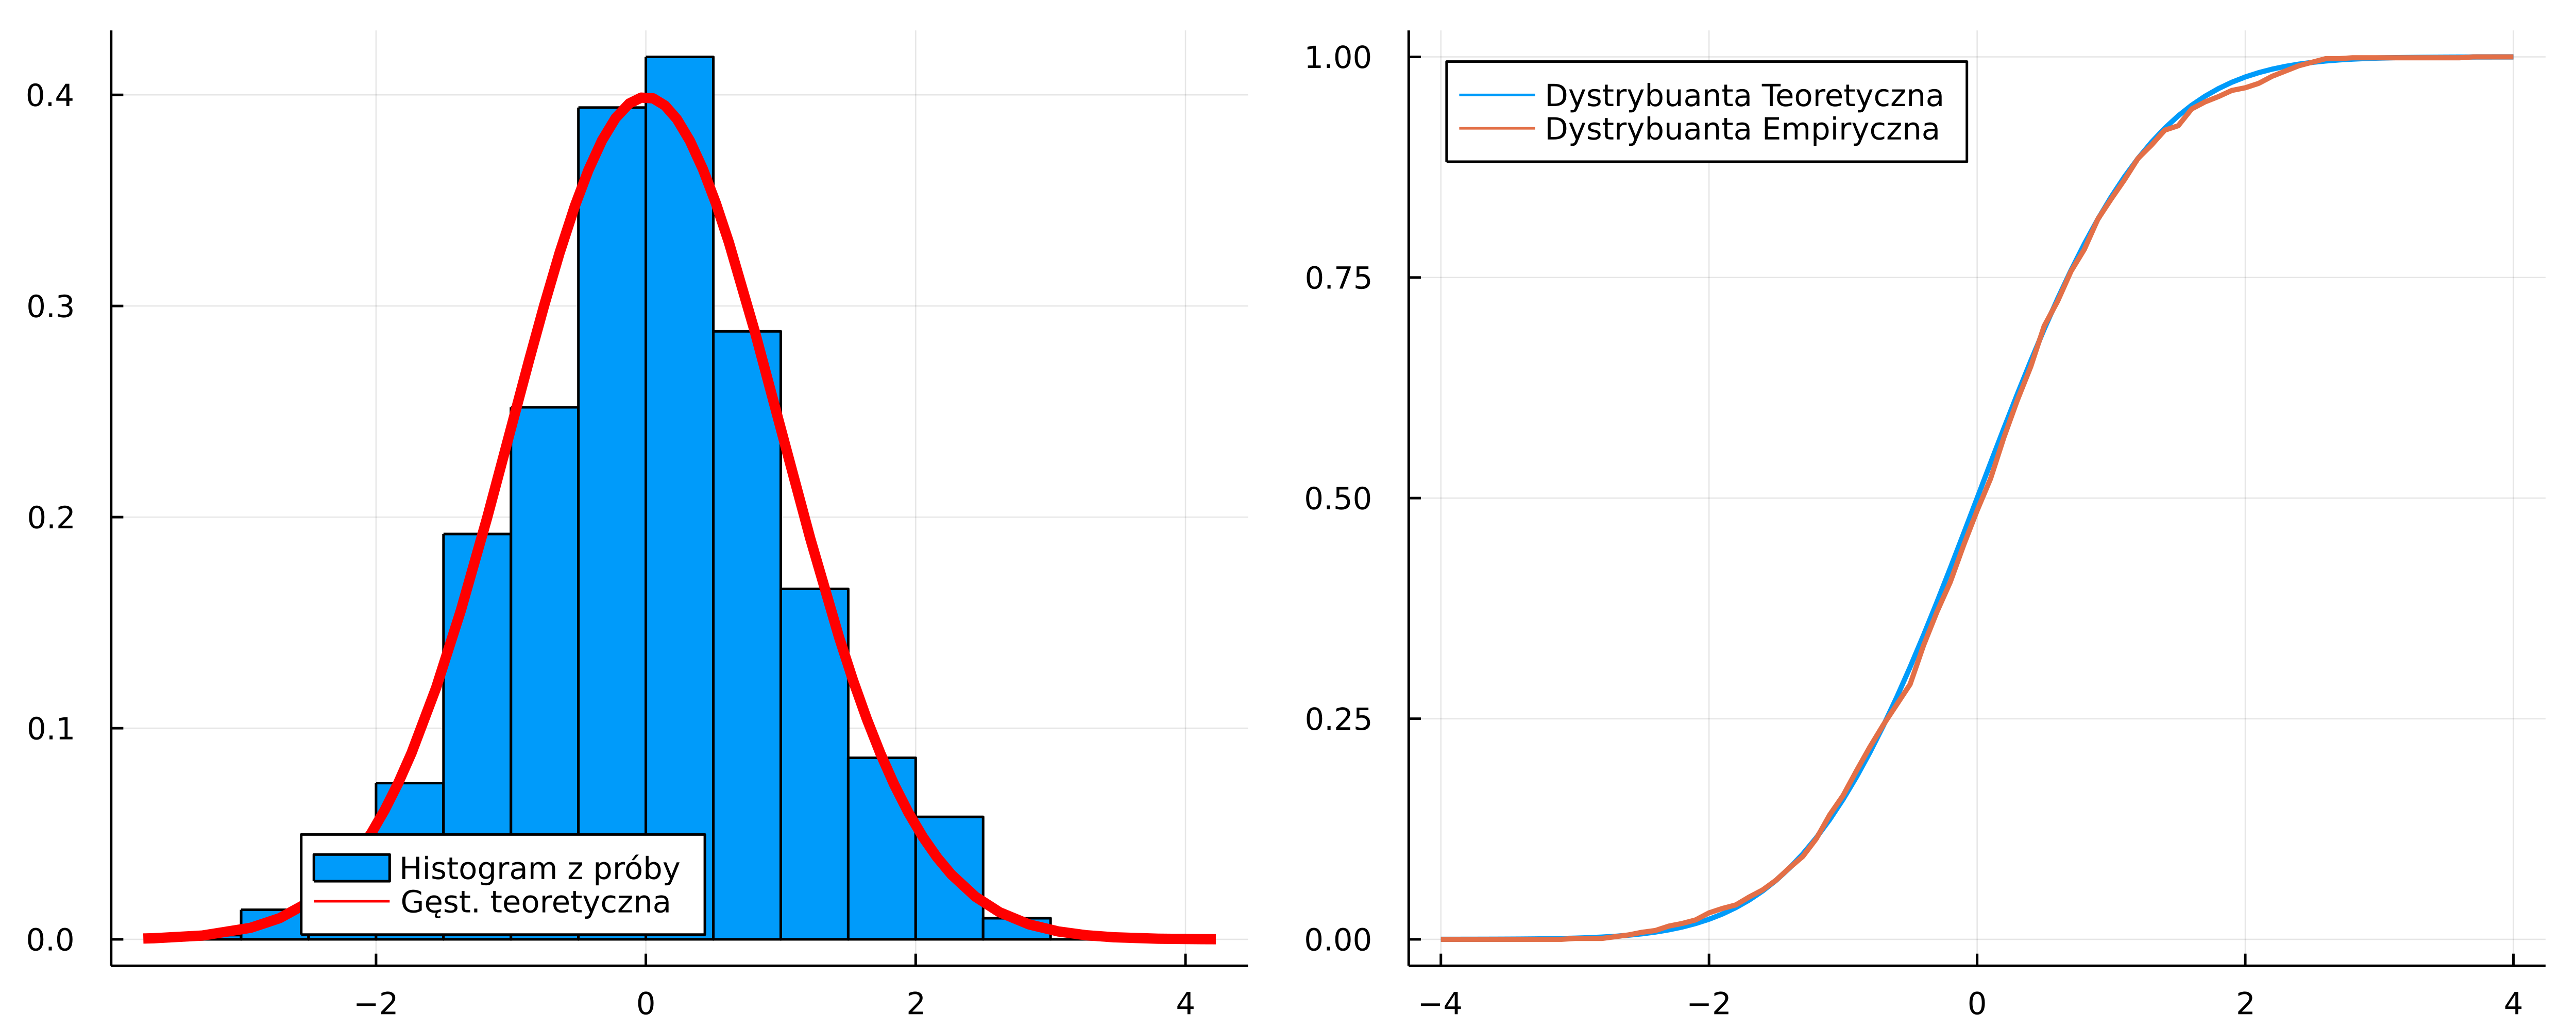
\includegraphics[width=\columnwidth]{fig/fig_BM.png}
	\end{figure}
	
	
	
	\section{Metoda biegunowa\textsuperscript{\cite{polar}} - Budink}
	\subsection{Opis}
	Jak wspomnieliśmy poprzednio rozkład normalny jest najważniejszym rozkładem prawdopodobieństwa. Z tego powodu jest on bardzo często wykorzystywany, ważne jest by generowanie próby trwało jak najkrócej. Niestety w metodzie Boxa-M{\"u}llera wyznaczanie pojawiają się funkcje $\sin$ oraz $\cos$. Wyznaczenie ich wartości jest stosunkowo czasochłonne dla procesora, dlatego była poszukiwana metoda, w która nie zawiera tych funkcji. Przekształcając wzór wykorzystywany w metodzie Boxa-M\"ullera można pokazać, że jeśli wektor $(V_1, V_2)$ ma rozkład jednostajny na kole jednostkowym to zmienne
	\begin{equation}
		\begin{split}
			X=\sqrt{\frac{-2\ln R^2}{R^2}}V_1\\
			Y=\sqrt{\frac{-2\ln R^2}{R^2}}V_2
		\end{split}
	\end{equation}
	mają rozkład normalny standardowy $\mathcal{N}(0,1)$ oraz $X \indep Y$. Ponieważ umiemy w sposób efektywny generować wektor losowy $(V_1, V_2)$ wystarczy skorzystać z poniższego algorytmu
	\subsubsection{Algorytm}
	\begin{enumerate}[leftmargin=10mm]
		\item Generuj zmienne $V_1, V_2$ - iid, $V_1\sim\mathcal{U}(-1,1)$
		\item Wyznacz $R^2=V_1^2+V_2^2$
		\item Jeżeli $R^2\ge 1$ wróć do 1.
		\item Zwróć
		\begin{equation}
			\begin{split}
				X=\sqrt{\frac{-2\ln R^2}{R^2}}V_1\\
				Y=\sqrt{\frac{-2\ln R^2}{R^2}}V_2
			\end{split}
		\end{equation}
	\end{enumerate}
	Podobnie jak w metodzie Boxa-M{\"u}llera algorytm ten zwraca dwie zmienne niezależne z rozkładu normalnego, więc by otrzymać zmienne z rozkładu $\mathcal{N}(\mu,\sigma^2)$ tak samo jak wcześniej mnożymy wygenerowaną próbę przez $\sigma$ i dodajemy do niej $\mu$.
	
	\subsection{Szybkość algorytmu}
	Do wygenerowania dwóch prób rozkładu normalnego korzystając z tego algorytmu potrzebne jest powtórzenie go średnio $\frac{4}{\pi}\approx1.25$ razy. Pomimo, że algorytm będzie czasem wykonywany wielokrotnie, to poprzez pozbycie się funkcji trygonometrycznych czas rzeczywisty wygenerowania danej próby będzie krótszy niż w poprzedniej metodzie, co pokażemy później.
	
	\subsection{Przykłady}

	\begin{figure}[H]\caption{Sprawdzenie poprawności metody biegunowej dla próby o rozmiarze $n=1000$}\label{fig:pol}
		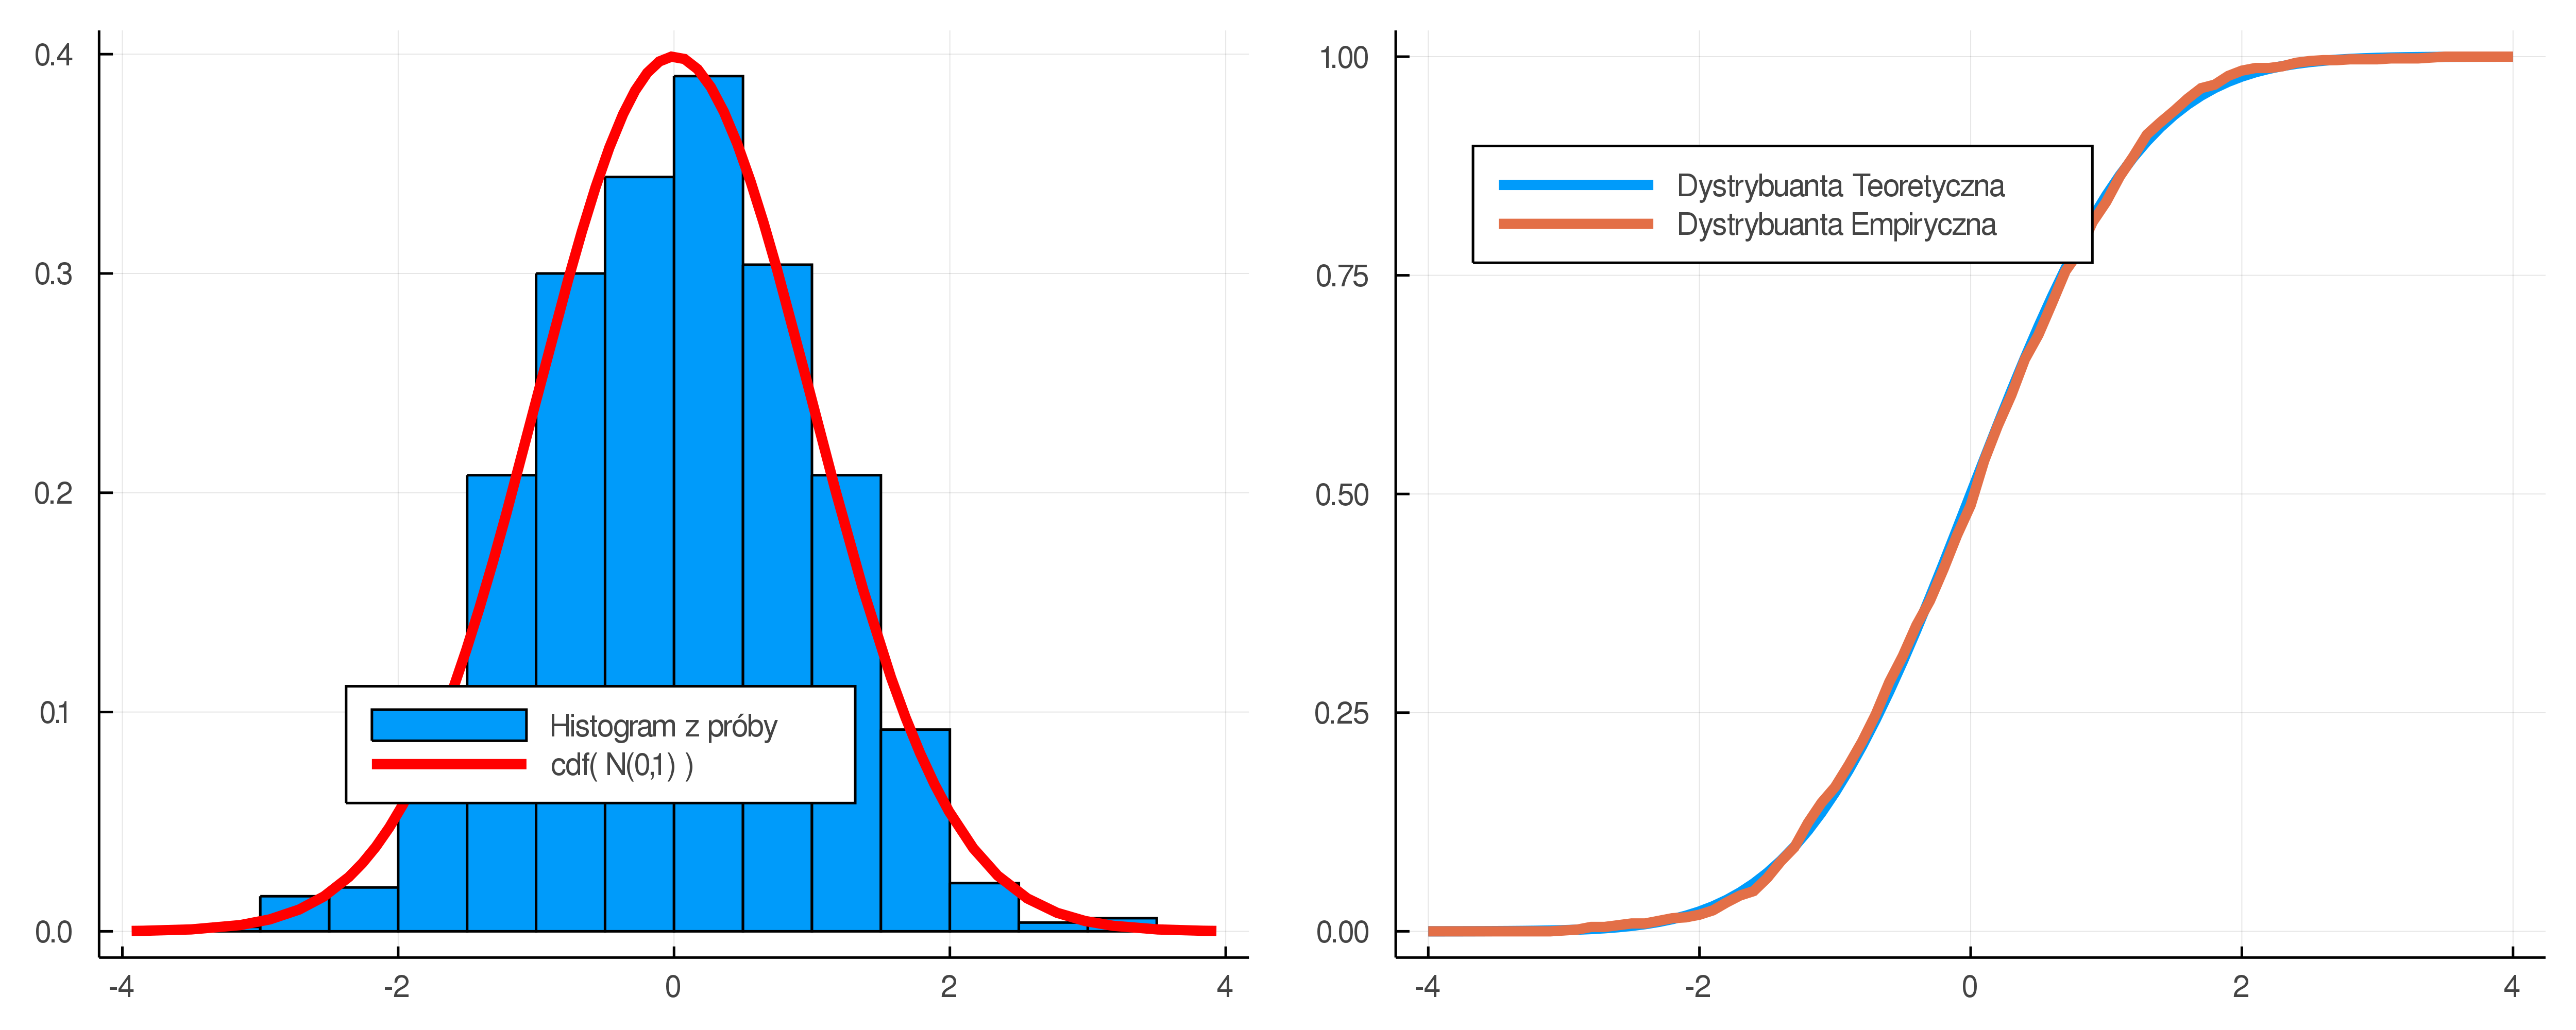
\includegraphics[width=\columnwidth]{fig/fig_pol.png}
	\end{figure}

	\section{Porównanie metod generowania rozkładu normalnego}
	Dwie ostatnie metody jakie pokazaliśmy dotyczą generowania tego samego rozkładu, dlatego ważne wydaje się, by porównać czas ich działania. Wykonaliśmy pomiary czasu generowania różnych wielkości prób (o wielkości $N$) dla metody Boxa-M\"ullera (B-M) oraz metody biegunowej. Dodatkowo policzyliśmy stosunek czasu potrzebnego do wygenerowania próby metodą biegunową do czasu B-M.
	\begin{table}[H]\caption{Czas wykonania danych metod dla danych wartości czasowych}\label{tab:time}
		\begin{tabularx}{\textwidth}{|Z{6mm}|Y|Z{19mm}|Y|p{5mm}|Z{6mm}|Y|Z{19mm}|Y|}
			\cline{1-4}\cline{6-9}
			$N$      & B-M &Biegunowa&stosunek& $\vphantom{\dfrac{1}{1}}$ & $N$      & B-M     &Biegunowa& stosunek \\ \cline{1-4}\cline{6-9}
			$2^{13}$ & 0.003 & 0.002 & 0.667 & $\vphantom{\dfrac{1}{1}}$ & $2^{22}$ & 0.113   & 0.052   & 0.46     \\ \cline{1-4}\cline{6-9}
			$2^{14}$ & 0.005 & 0.004 & 0.800 & $\vphantom{\dfrac{1}{1}}$ & $2^{23}$ & 0.371   & 0.226   & 0.609    \\ \cline{1-4}\cline{6-9}
			$2^{15}$ & 0.009 & 0.009 & 1.000 & $\vphantom{\dfrac{1}{1}}$ & $2^{24}$ & 0.741   & 0.522   & 0.704    \\ \cline{1-4}\cline{6-9}
			$2^{16}$ & 0.019 & 0.013 & 0.684 & $\vphantom{\dfrac{1}{1}}$ & $2^{25}$ & 1.180   & 1.199   & 1.016    \\ \cline{1-4}\cline{6-9}
			$2^{17}$ & 0.030 & 0.019 & 0.633 & $\vphantom{\dfrac{1}{1}}$ & $2^{26}$ & 2.121   & 1.571   & 0.741    \\ \cline{1-4}\cline{6-9}
			$2^{18}$ & 0.019 & 0.003 & 0.158 & $\vphantom{\dfrac{1}{1}}$ & $2^{27}$ & 3.996   & 2.863   & 0.716    \\ \cline{1-4}\cline{6-9}
			$2^{19}$ & 0.013 & 0.013 & 1.000 & $\vphantom{\dfrac{1}{1}}$ & $2^{28}$ & 7.643   & 4.244   & 0.555    \\ \cline{1-4}\cline{6-9}
			$2^{20}$ & 0.028 & 0.015 & 0.536 & $\vphantom{\dfrac{1}{1}}$ & $2^{29}$ & 38.264  & 9.015   & 0.236    \\ \cline{1-4}\cline{6-9}
			$2^{21}$ & 0.056 & 0.028 & 0.500 & $\vphantom{\dfrac{1}{1}}$ & $2^{30}$ & 308.305 & 125.324 & 0.406    \\ \cline{1-4}\cline{6-9}
		\end{tabularx}
	\end{table}
	\textbf{Rośnie wykładniczo, trzeba powtórzyć kilkukrotnie dla danej wielkości $N$}

	
	\section{Zakończenie - Początek}
	
	
	\begin{thebibliography}{1}
		\bibitem{AO - dyskretny}
		\url{https://youtu.be/NFmbgbyj5M0?t=1323}
		
		\bibitem{AO - ciagly}
		\url{https://youtu.be/SpPS0CnhvrE?t=37}
		
		\bibitem{splot}
		\url{https://youtu.be/SpPS0CnhvrE?t=4081}
		
		\bibitem{kompozycja}
		\url{https://youtu.be/7lOH982wrwo?t=50}
		
		\bibitem{box-kox}
		\url{https://youtu.be/7lOH982wrwo?t=1896}
		
		\bibitem{polar}
		\url{https://youtu.be/7lOH982wrwo?t=3349}

	\end{thebibliography}
	
\end{document}